
\chapter{完全随机实验中的内曼重复抽样推断}\label{chapter::neyman-cr}
 \chaptermark{完全随机实验与内曼推断}
 
 
在具有里程碑意义的论文中，\citet{Neyman:1923}不仅提出了潜在结果的概念，还推导出了在完全随机实验条件下对平均因果效应进行推断的严格数学结论。与费希尔在尖锐零假设下计算$p$值的思想不同，\citet{Neyman:1923}提出了一种无偏点估计量，以及基于该估计量抽样分布得到的保守置信区间。本章将介绍\citet{Neyman:1923}的这些基础性结论，它们对于理解本书\ref{part::rcts}部分后续章节至关重要。



\section{有限总体中的统计量}

考虑包含$n$个单位的完全随机实验，其中$n_1$个接受处理，$n_0$个作为对照。单位$i = 1, \ldots, n$的潜在结果为$Y_i(1)$和$Y_i(0)$，个体效应为$\tau_i = Y_i(1) - Y_i(0).$。潜在结果的有限总体均值为
$$
\bar{Y}(1) = n^{-1} \sumn Y_i(1),\quad
\bar{Y}(0) = n^{-1} \sumn Y_i(0),
$$
方差为\footnote{以$n-1$为除数可使本章主要定理更简洁。改用$n$会使公式复杂，但不改变基本结论；$n$较大时，差异很小。}
$$
S^2(1) = (n-1)^{-1} \sumn \{ Y_i(1) -\bar{Y}(1)  \}^2,\quad
S^2(0) = (n-1)^{-1} \sumn \{ Y_i(0) -\bar{Y}(0)  \}^2 ,
$$
协方差为
$$
S(1,0) = (n-1)^{-1} \sumn \{ Y_i(1) -\bar{Y}(1)  \}\{ Y_i(0) -\bar{Y}(0)  \} . 
$$
个体效应的均值为
$$
\tau = n^{-1} \sumn \tau_i = \bar{Y}(1) - \bar{Y}(0) .
$$
方差为
$$
S^2(\tau) = (n-1)^{-1} \sumn (\tau_i - \tau)^2.
$$
这些方差与协方差满足以下关系。
\begin{lemma}\label{lemma::variancecovariancetau}
$2S(1,0) = S^2(1)+S^2(0) - S^2(\tau).$
\end{lemma}

引理\ref{lemma::variancecovariancetau}是后续讨论要用到的基本结论。引理\ref{lemma::variancecovariancetau}可通过初等代数证明，留作习题\ref{hw::proof-covariance-basic}。 

这些统计量均由科学表$\{ Y_i(1), Y_i(0)  \}_{i=1}^n$所决定。我们感兴趣的是：基于完全随机实验中观测到的数据$ (Z_i, Y_i)_{i=1}^n$，如何估计平均因果效应$\tau$。 


\section{\citet{Neyman:1923}的定理}


根据观测结果，可计算样本均值
$$
\hat{\bar{Y}}(1) = n_1^{-1} \sumn Z_i Y_i,\quad
\hat{\bar{Y}}(0) = n_0^{-1} \sumn (1-Z_i) Y_i,
$$
与样本方差
$$
\hat{S}^2(1) = (n_1 - 1)^{-1} \sumn Z_i  \{  Y_i - \hat{\bar{Y}}(1) \}^2,\quad
\hat{S}^2(0) = (n_0 - 1)^{-1} \sumn (1-Z_i)  \{  Y_i - \hat{\bar{Y}}(0) \}^2 . 
$$
但$S(1,0)$与$S^2(\tau)$没有可计算的样本版本，因为每个单位$i$的潜在结果$Y_i(1)$和$Y_i(0)$永远不能同时观测。\citet{Neyman:1923}证明了以下定理。 




\begin{theorem}
\label{thm::neyman1923}
在完全随机实验条件下， 
\begin{enumerate}
\item
均值差估计量$\hat{\tau} =\hat{\bar{Y}}(1) -  \hat{\bar{Y}}(0)$是$\tau$的无偏估计量：
$$
E(\hat{\tau}) =\tau ;
$$ 
\item
$\hat{\tau} $的方差为
\begin{eqnarray}
\var(\hat{\tau})  &=&  \frac{S^2(1)}{n_1} + \frac{S^2(0)}{n_0} - \frac{S^2(\tau)}{n} \label{eq::neyman23var} \\
&=& \frac{n_0}{n_1 n} S^2(1) + \frac{n_1}{n_0 n} S^2(0) + \frac{2}{n} S(1,0) ;  \label{eq::neyman23var-equivalent}
\end{eqnarray}
\item\label{neyman-3}
方差估计量 
$$
\hat{V} = \frac{\hat{S}^2(1)}{n_1} + \frac{\hat{S}^2(0)}{n_0}
$$
是$\var(\hat{\tau})$的一个保守估计量，即满足
$$
E(\hat{V} ) - \var(\hat{\tau})  = \frac{S^2(\tau)}{n}  \geq 0
$$
当且仅当所有单位的$\tau_i = \tau$时等号成立。 
\end{enumerate}
\end{theorem}

定理\ref{thm::neyman1923}的证明见第\ref{sec::prove-neyman-1923}节。在证明定理\ref{thm::neyman1923}之前，必须澄清定理\ref{thm::neyman1923}中$E(\cdot)$与$\var(\cdot)$的含义。潜在结果均固定，只有处理指标$Z_i$随机。因此，期望与方差都针对各$Z_i$的随机性计算；处理向量是$n_1$个 1 与$n_0$个 0 的随机排列。图\ref{fig::neyman1923}说明$\hat\tau$的随机性：$M=\binom{n}{n_1}$种处理分配等概率出现，分别对应$\{ \hat\tau^1 , \ldots, \hat\tau^M\}$中的取值，从而诱导其抽样分布。比较图\ref{fig::neyman1923}与图\ref{fig::frt}，可见 FRT 与\citet{Neyman:1923}定理的关键区别：
\begin{enumerate}
\item
FRT 适用于任意检验统计量，\citet{Neyman:1923}的定理则只针对均值差。虽然也可为其他估计量推导类似\citet{Neyman:1923}的结论，但对一般估计量而言，数学推导往往很困难。 

\item
图\ref{fig::frt}中观测结果向量$\bm{Y}$是固定不变的，而图\ref{fig::neyman1923}中$\bm{Y}(\bm{z}^m)$的值随处理分配方案$\bm{z}^m$变化。 

\item
图\ref{fig::frt}中各$T(\bm{z}^m,\bm{Y}) $均可由观测数据计算，图\ref{fig::neyman1923}中各$\hat\tau^m$却是假想值，因为并非所有潜在结果都已知。 
\end{enumerate}

\begin{figure}[ht]
\centering 
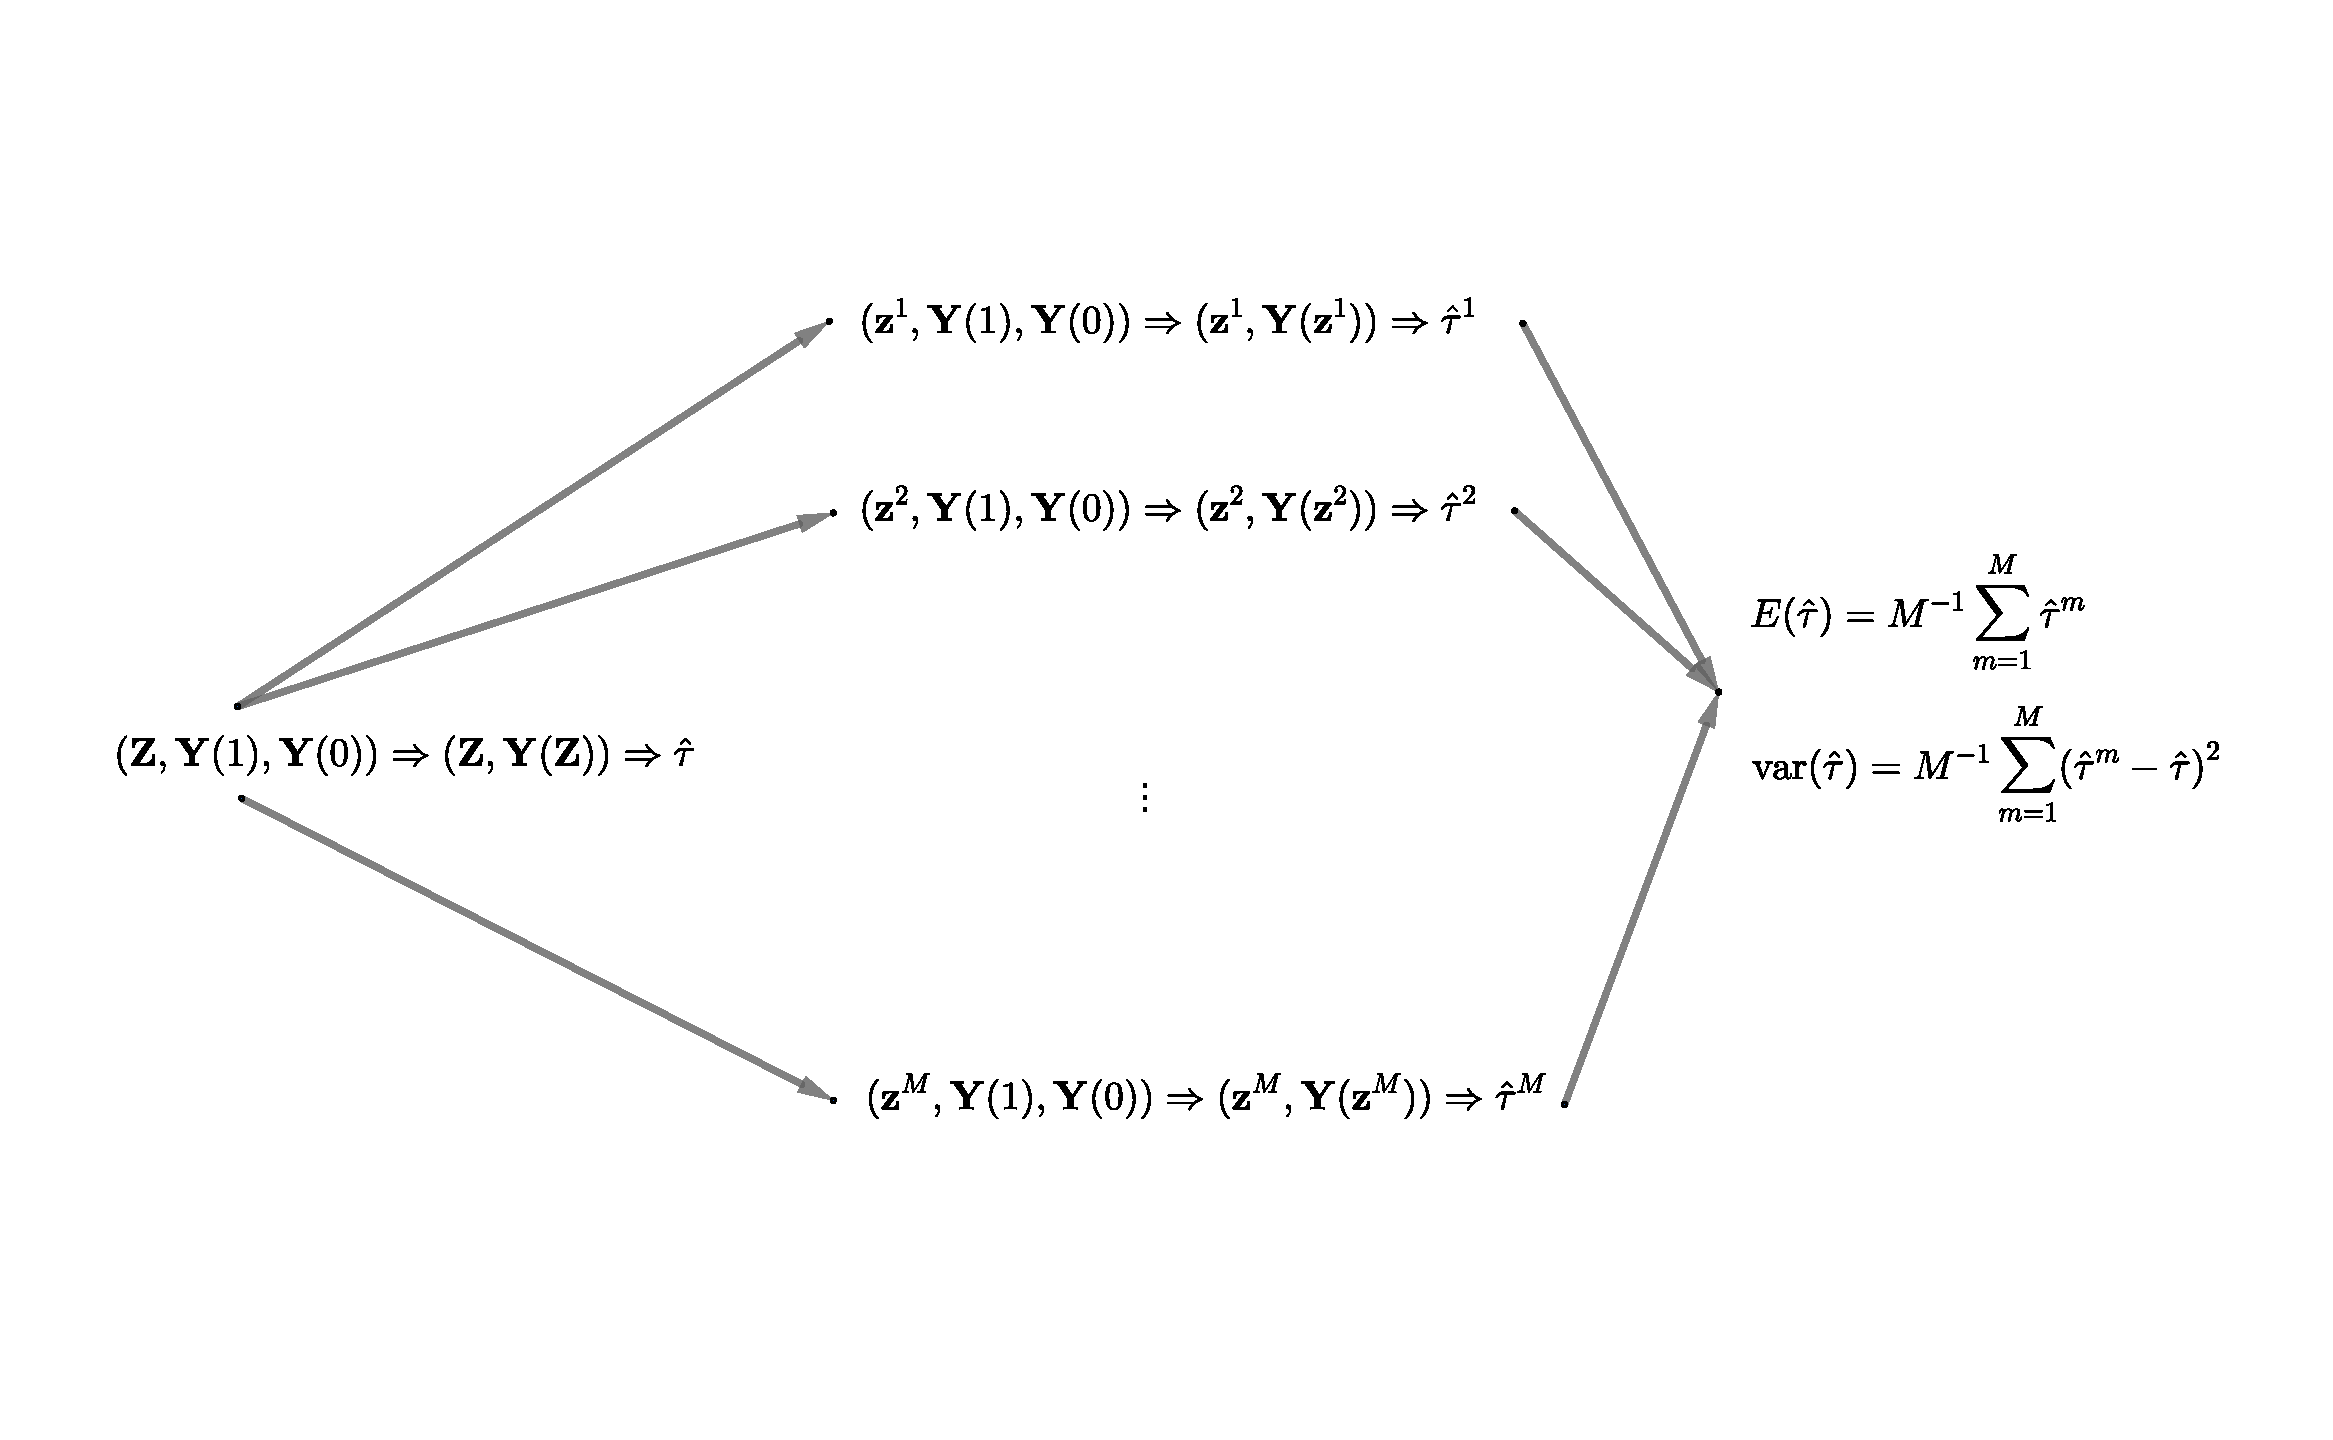
\includegraphics[width =  \textwidth]{figures/neyman1923_fig.pdf}
\caption{\citet{Neyman:1923}定理示意图，其中$\bm{Y}(\bm{z}^m)$为给定处理分配方案$\bm{z}^m$时的观测结果向量。}\label{fig::neyman1923}
\end{figure}




点估计量$\hat\tau$虽然形式简单，但在完全随机实验框架下其方差却具有非平凡特性。式\eqref{eq::neyman23var}所示的方差表达式与经典均值差方差公式\footnote{在经典双样本问题中，处理组观测值独立同分布于均值$\mu_1$、方差$\sigma_1^2$的分布，对照组观测值独立同分布于均值$\mu_0$、方差$\sigma_0^2$的分布。此时有
$$
\var(\hat{\tau} ) = \frac{\sigma_1^2}{n_1} +  \frac{\sigma_0^2}{n_0}.
$$
此处$\var(\cdot)$均指观测值的随机性。该公式不含涉及个体因果效应方差的第三项。}存在显著差异：它不仅取决于潜在结果的有限总体方差，还包含个体处理效应方差（或等价的潜在结果协方差）。遗憾的是，由于$Y_i(1)$与$Y_i(0)$无法同时观测，因此$S^2(\tau)$与$S(1,0)$均无法由数据直接识别。 




公式\eqref{eq::neyman23var}有些令人困惑：个体效应越异质，$\hat{\tau}$的变异反而越小。第\ref{sec::simulation-neyman-formula}节将用数值例子验证\eqref{eq::neyman23var}。直观原因是什么？可以根据等价形式\eqref{eq::neyman23var-equivalent}，比较潜在结果正相关与负相关的情形。处理组虽然是从$n$个单位的有限总体中简单随机抽取的，一次实际实验仍可能恰好选到处理潜在结果较大的单位。假设出现了这种情况。 
\begin{enumerate}
\item
若$S(1,0) > 0$，这些处理单位的对照潜在结果也较大，剩余对照单位的观测结果因而较小，使$\hat\tau$较大。 
\item
若$S(1,0) < 0$，这些处理单位的对照潜在结果较小，剩余对照单位的观测结果因而较大，使$\hat\tau$较小。 
\end{enumerate}
若某次实验恰好选到处理潜在结果较小的单位，也会出现方向相反的情况。总之，$\hat\tau$的无偏性不依赖潜在结果的相关性，但与$S(1,0) < 0$相比，在$S(1,0) > 0$下更容易观测到极端的$\hat\tau$。因此，潜在结果正相关时，$\hat{\tau}$的方差更大。 

 
 
 
 


\citet[][Theorem 5 and Proposition 3]{li2017general}基于有限总体中心极限定理，进一步证明了$\hat{\tau}$的以下渐近正态性。
\begin{theorem}
\label{thm::clt-difference-in-means}
设$n\rightarrow \infty$且$n_1 \rightarrow \infty$。若$n_1/n$收敛于$(0,1)$区间内的某定值，$\{S^2(1), S^2(0), S(1,0)\}$亦存在极限值，且满足
$$  
\max_{1\leq i \leq n}\{ Y_i(1) - \bar{Y}(1) \}^2/n \rightarrow 0, \quad 
\max_{1\leq i \leq n}\{ Y_i(0) - \bar{Y}(0) \}^2/n \rightarrow 0,
$$
则
$$
\frac{   \hat{\tau} - \tau }{  \sqrt{ \var(\hat{\tau}) } } \rightarrow \N01
$$
依分布收敛，同时
$$
\hat{S}^2(1) \rightarrow S^2(1),\quad 
\hat{S}^2(0) \rightarrow S^2(0)
$$
依概率收敛。 
\end{theorem}


定理\ref{thm::clt-difference-in-means}的证明涉及较多技术细节，超出本书范围。它保证在大样本及一定正则条件下，$\hat{\tau} $的抽样分布可用正态分布近似；结果的样本方差也一致估计总体方差，从而使\cite{Neyman:1923}方差估计的概率极限不低于$\hat{\tau} $的真实方差。因此，可构造$\tau$的保守大样本置信区间：
$$
\hat{\tau} \pm z_{1-\alpha/2} \sqrt{  \hat{V}  },
$$
其中$z_{1-\alpha/2}$为标准正态分布的$1-\alpha/2$分位数。这与标准双样本问题的置信区间渐近相同（见第\ref{sec::bf-problem}节）。样本量足够大时，该区间覆盖$\tau$的概率至少为$1-\alpha$。由对偶性，可据此检验
$$
\HN: \tau = 0,
$$
这称为弱零假设。 



由于潜在结果缺失的根本性限制，我们只能获得保守型方差估计量。统计学中置信区间的定义本身即允许覆盖率超标的存在，这也使得方差估计的保守性具有合理性（参见\ref{sec::statistical-inference}节）。若实际研究中对处理效应估计不足的危害可控，这种保守性便无大碍。但当研究涉及药物副作用测量时，估计不足可能带来严重危害——例如新药的毒性效应若被低估将危及患者健康。 
 
 

\section{证明}\label{sec::prove-neyman-1923}

本节将完整证明定理\ref{thm::neyman1923}。


首先，$\hat{\tau}$的无偏性可直接由如下展开式与期望线性性质推导：
\begin{eqnarray*}
\hat{\tau} &=& n_1^{-1} \sumn Z_i Y_i - n_0^{-1} \sumn (1-Z_i) Y_i \\
&=& n_1^{-1} \sumn Z_i Y_i(1) - n_0^{-1} \sumn (1-Z_i) Y_i(0) 
\end{eqnarray*}
于是
\begin{eqnarray*}
E( \hat{\tau}  ) &=& E\left\{    n_1^{-1} \sumn Z_i Y_i(1) - n_0^{-1} \sumn (1-Z_i) Y_i(0)   \right\} \\
&=& n_1^{-1} \sumn E(Z_i) Y_i(1) - n_0^{-1} \sumn E(1-Z_i) Y_i(0) \\
&=& n_1^{-1} \sumn \frac{n_1}{n} Y_i(1) - n_0^{-1} \sumn \frac{n_0}{n} Y_i(0) \\
&=&  n^{-1} \sumn Y_i(1) - n^{-1} \sumn Y_i(0) \\
&=& \tau .
\end{eqnarray*}


第二，将$\hat{\tau}$进一步改写为
\begin{eqnarray*}
\hat{\tau} &=&  \sumn Z_i  \left\{    \frac{  Y_i(1) }{ n_1 } + \frac{  Y_i(0) }{ n_0 }   \right\}
- n_0^{-1} \sumn Y_i(0).
\end{eqnarray*}
根据简单随机抽样的引理\ref{lemma::samplemean}，$\hat{\tau}$的方差为
\begin{eqnarray*}
\var(\hat{\tau}) &=&  \frac{  n_1 n_0  }{  n(n-1)  }  \sumn  
\left\{    \frac{  Y_i(1) }{ n_1 } + \frac{  Y_i(0) }{ n_0 }  -  \frac{  \bar{Y}(1) }{ n_1 } - \frac{  \bar{Y}(0) }{ n_0 }    \right\}^2 \\
&=&  \frac{  n_1 n_0  }{  n(n-1)  }  \left[
\frac{1}{n_1^{2}}   \sumn  \{  Y_i(1) -  \bar{Y}(1)\}^2 + \frac{1}{n_0^{2}}  \sumn  \{  Y_i(0) -  \bar{Y}(0)\}^2 \right. \\
&& \left. \qquad \qquad 
+ \frac{2}{n_1 n_0}  \sumn  \{  Y_i(1) -  \bar{Y}(1)\}  \{  Y_i(0) -  \bar{Y}(0)\} 
\right]\\
&=& \frac{n_0}{n_1n} S^2(1) + \frac{n_1}{n_0n}S^2(0) + \frac{2}{n} S(1,0). 
\end{eqnarray*}
由引理\ref{lemma::variancecovariancetau}，还可将方差写为
\begin{eqnarray*}
\var(\hat{\tau})
&=& \frac{n_0}{n_1n} S^2(1) + \frac{n_1}{n_0n}S^2(0) + \frac{1}{n} \{ S^2(1)+S^2(0) - S^2(\tau) \}\\
&=&  \frac{S^2(1)}{n_1} + \frac{S^2(0)}{n_0} - \frac{S^2(\tau)}{n}.
\end{eqnarray*}

第三，处理组是从$n$个单位中抽取的大小为$n_1$的简单随机样本。因此，由引理\ref{lemma::variance-unbiased}，各$Y_i(1)$的样本方差无偏估计总体方差：
$$
E\{  \hat{S}^2(1) \} = S^2(1).
$$
类似地，$E\{  \hat{S}^2(0) \} = S^2(0).$。所以$\hat{V} $是\eqref{eq::neyman23var}前两项之和的无偏估计。 
 
 
 
 
 \section{完全随机实验的回归分析}
 
 
 
实践中常用回归对平均因果效应$\tau$作推断。标准做法是将结果对处理指标及截距作普通最小二乘（OLS）回归：
$$
(\hat\alpha, \hat\beta) = \arg\min_{(a,b)} \sum_{i=1}^n (Y_i - a - bZ_i)^2,
$$
以处理系数$ \hat\beta$估计平均因果效应。可以证明，$ \hat\beta$恰好等于均值差：
\begin{equation}
\label{eq::ols-difference-in-means}
\hat\beta = \hat\tau .
\end{equation}

但 OLS 的通常方差估计量（见第\ref{appendix::basic-linear-regression}章的\eqref{eq::v-hat-ols}），例如\ri{R}中\ri{lm}函数的输出，等于
\begin{eqnarray}
\label{eq::ols-se}
\hat V_\textsc{ols} &=& \frac{n\left(n_1 -1\right)}{( n-2 ) n_1  n_0 } \hat S^2(1) +\frac{n\left(n_0 -1\right)}{( n-2 ) n_1  n_0 } \hat S^2(0)\\
\nonumber &\approx& \frac{\hat S^2(1)}{n_0 }+\frac{ \hat S^2(0) }{n_1 },
\end{eqnarray}
近似在$ n_1 $和$ n_0 $较大时成立。即使$ n_1 $、$ n_0 $很大，它仍不同于$\hat{V}$。 


幸运的是，Eicker--Huber--White（EHW）稳健方差估计量（见第\ref{appendix::basic-linear-regression}章的\eqref{eq::v-hat-ehw}）接近$\hat{V}$：
\begin{eqnarray}
\label{eq::ols-ehw}
\hat V_\textsc{ehw} &=& \frac{\hat S^2(1)}{n_1 } \frac{n_1 -1}{n_1 }+\frac{\hat S^2(0)}{n_0 } \frac{n_0 -1}{n_0 } \\
\nonumber &\approx& \frac{ \hat S^2(1)  }{n_1 }+\frac{ \hat S^2(0) }{n_0 }
\end{eqnarray}
近似在$ n_1 $和$ n_0 $较大时成立，几乎等于$\hat{V}$。而且，EHW 稳健方差估计的 HC2 变体与$\hat{V}$完全相同。\ri{car}包中的\ri{hccm}函数可以计算 EHW 稳健方差及 HC2 变体。 

习题\ref{hw::neyman-ols-nox}给出了\eqref{eq::ols-difference-in-means}至\eqref{eq::ols-ehw}的更多技术细节。 
 



 

 
\section{实例演示} 


\subsection{模拟}
\label{sec::simulation-neyman-formula}



首先设定样本总量$n=100$，其中处理组$60$例、对照组$40$例，生成个体效应恒定的潜在结果： 
\begin{lstlisting}
n  = 100
n1 = 60
n0 = 40
y0 = rexp(n)
y0 = sort(y0, decreasing = TRUE)
y1 = y0 + 1
 \end{lstlisting}
固定科学表，反复生成完全随机实验，并应用定理\ref{thm::neyman1923}计算点估计、保守方差估计以及基于正态近似的置信区间。图\ref{fig::simulation-neyman}的$(1,1)$子图给出潜在结果散点图，图\ref{fig::simulation-neyman}的$(1,2)$子图给出$\hat{\tau} - \tau$的直方图。 

随后反转对照组结果顺序重新模拟：
\begin{lstlisting}
y0 = sort(y0, decreasing = FALSE)
 \end{lstlisting}
并重复上述模拟。图\ref{fig::simulation-neyman}的$(2,1)$子图给出潜在结果散点图，图\ref{fig::simulation-neyman}的$(2,2)$子图给出$\hat{\tau} - \tau$的直方图。 




最后，随机置换对照潜在结果： 
 \begin{lstlisting}
y0 = sample(y0)
 \end{lstlisting}
 并重复上述模拟。图\ref{fig::simulation-neyman}的$(3,1)$子图给出潜在结果散点图，图\ref{fig::simulation-neyman}的$(3,2)$子图给出$\hat{\tau} - \tau$的直方图。 

 
 三组模拟中，潜在结果的相关性不同，但边际分布相同。下表比较真实方差、估计方差的平均值以及$95\%$置信区间的覆盖率。 
 \begin{lstlisting}
              constant negative independent
var              0.036    0.007       0.020
estimated var    0.036    0.036       0.036
coverege rate    0.947    1.000       0.989
 \end{lstlisting}
真实方差依赖潜在结果的相关性：潜在结果正相关时，抽样方差较大，验证了\eqref{eq::neyman23var-equivalent}。估计方差几乎相同，因为$\hat{V}$的公式只依赖潜在结果的边际分布。由于真实方差与估计方差不同，三组模拟的覆盖率也不同。只有因果效应恒定时，估计方差才在平均意义上等于真实方差，验证了定理\ref{thm::neyman1923}的第\ref{neyman-3}点。 
 
图\ref{fig::simulation-neyman}还画出了基于$\hat{\tau} $中心极限定理的正态密度曲线，与模拟直方图很接近，验证了定理\ref{thm::clt-difference-in-means}。
 
 
 \begin{figure}
 \centering 
 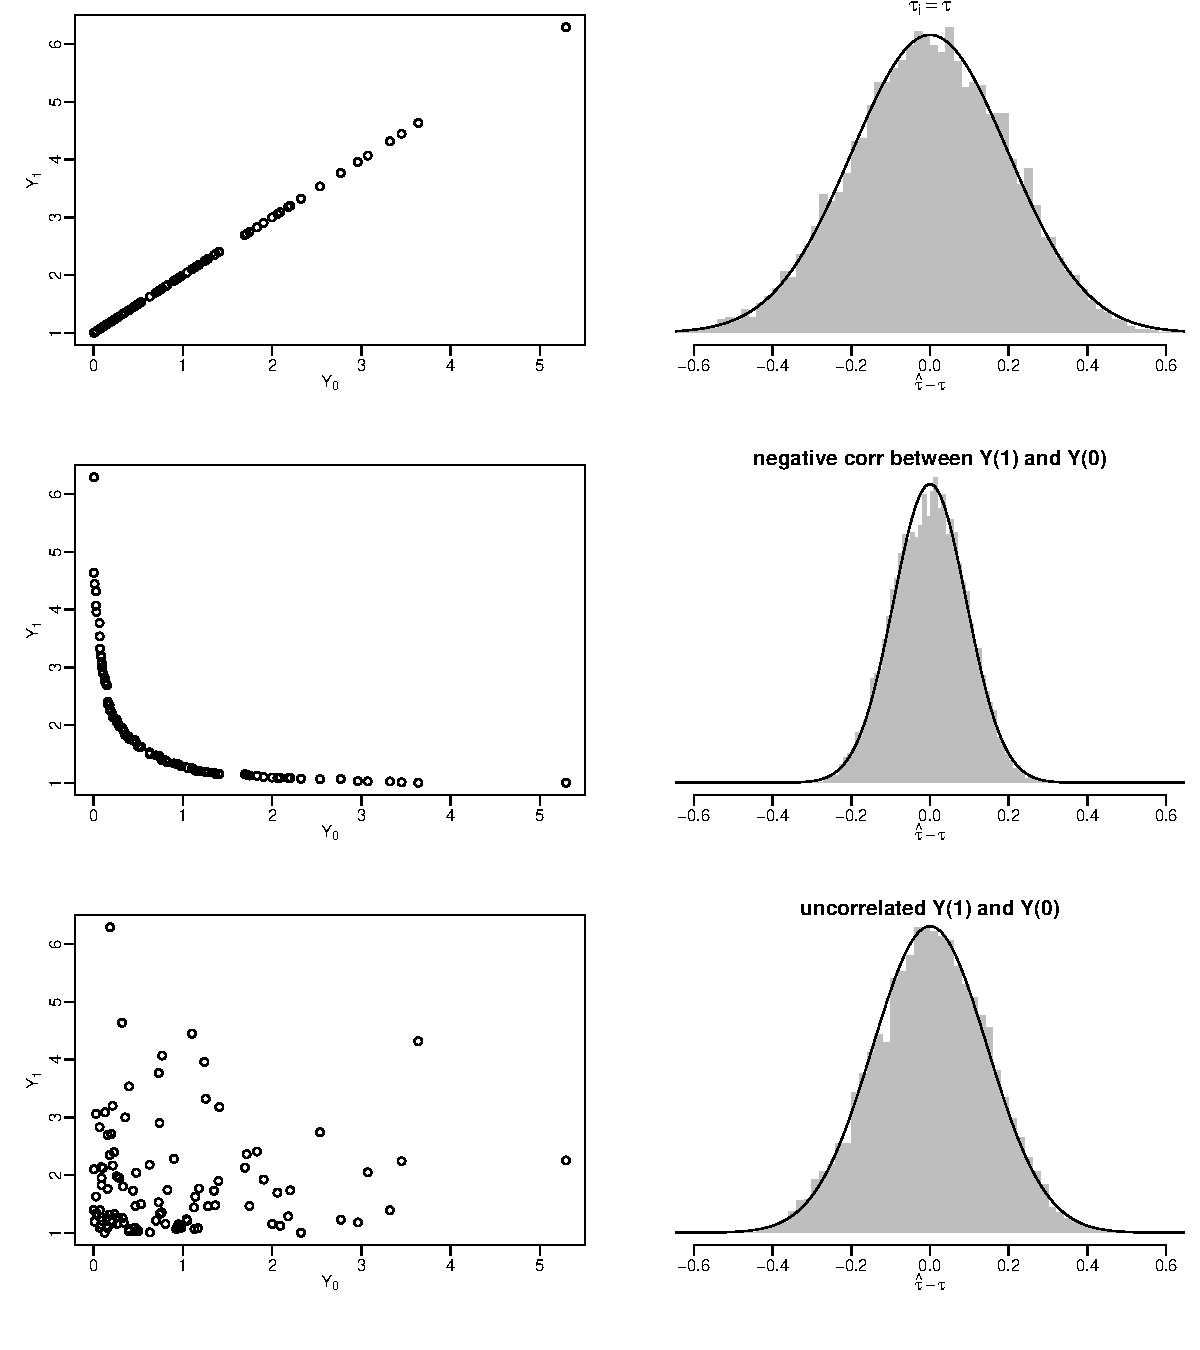
\includegraphics[width = \textwidth]{figures/neymanevaluation3.pdf}
 \caption{左：边际分布相同的潜在结果联合分布。右：不同潜在结果联合分布下，$10^4$次模拟所得$\hat{\tau} - \tau$的抽样分布。}\label{fig::simulation-neyman}
 \end{figure} 
 
 
 
 
 
 \subsection{重尾分布下的正态近似失效}


定理\ref{thm::clt-difference-in-means}中$\hat{\tau}  $的中心极限定理需要正则条件，重尾潜在结果会违反这些条件。可修改前面的模拟说明这一点：保持个体因果效应恒定，但让对照潜在结果以$0.1, 0.3$或$0.5$的概率受到柯西分布成分污染。下面的代码生成污染概率为$0.1$的潜在结果。 

\begin{lstlisting}
eps = rbinom(n, 1, 0.1)
y0 = (1 - eps)*rexp(n) + eps*rcauchy(n)
y1 = y0 + 1
\end{lstlisting} 


图\ref{fig::simulation-neyman-heavytail-1}和\ref{fig::simulation-neyman-heavytail-2}给出了两次实现中$\hat{\tau} - \tau$的直方图及对应正态近似。潜在结果呈重尾时，正态近似很差；而且与图\ref{fig::simulation-neyman}不同，直方图对模拟的随机种子很敏感。 


 \begin{figure}
 \centering 
 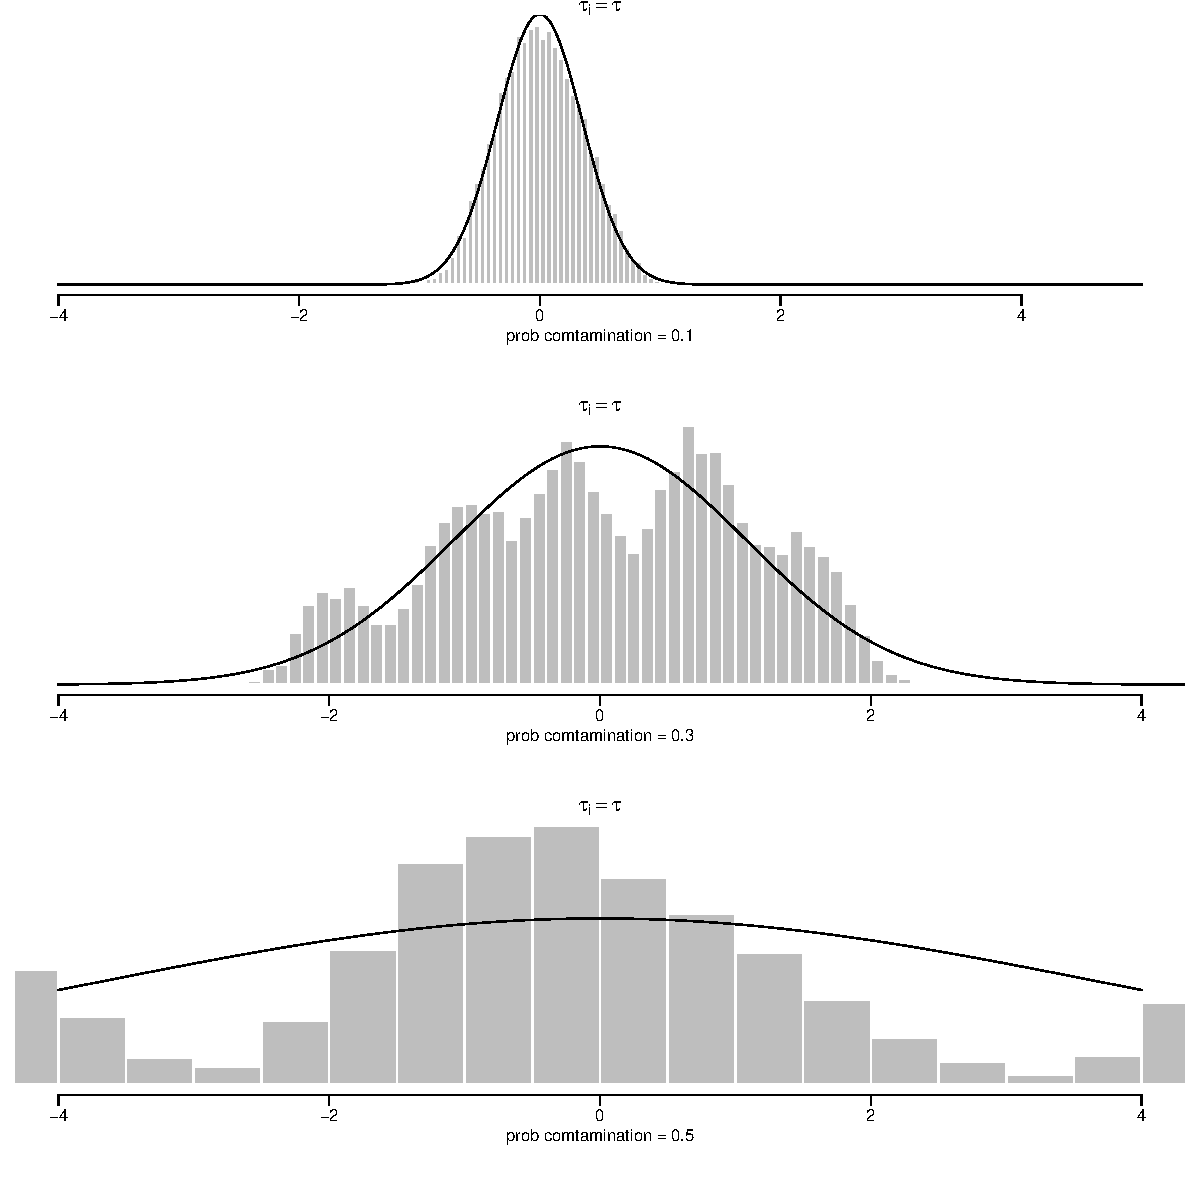
\includegraphics[width = \textwidth]{figures/neyman_comtamination_realized1.pdf}
 \caption{潜在结果受到不同概率污染时$\hat{\tau} - \tau$的抽样分布：第一次实现}\label{fig::simulation-neyman-heavytail-1}
 \end{figure} 
 
  \begin{figure}
 \centering 
 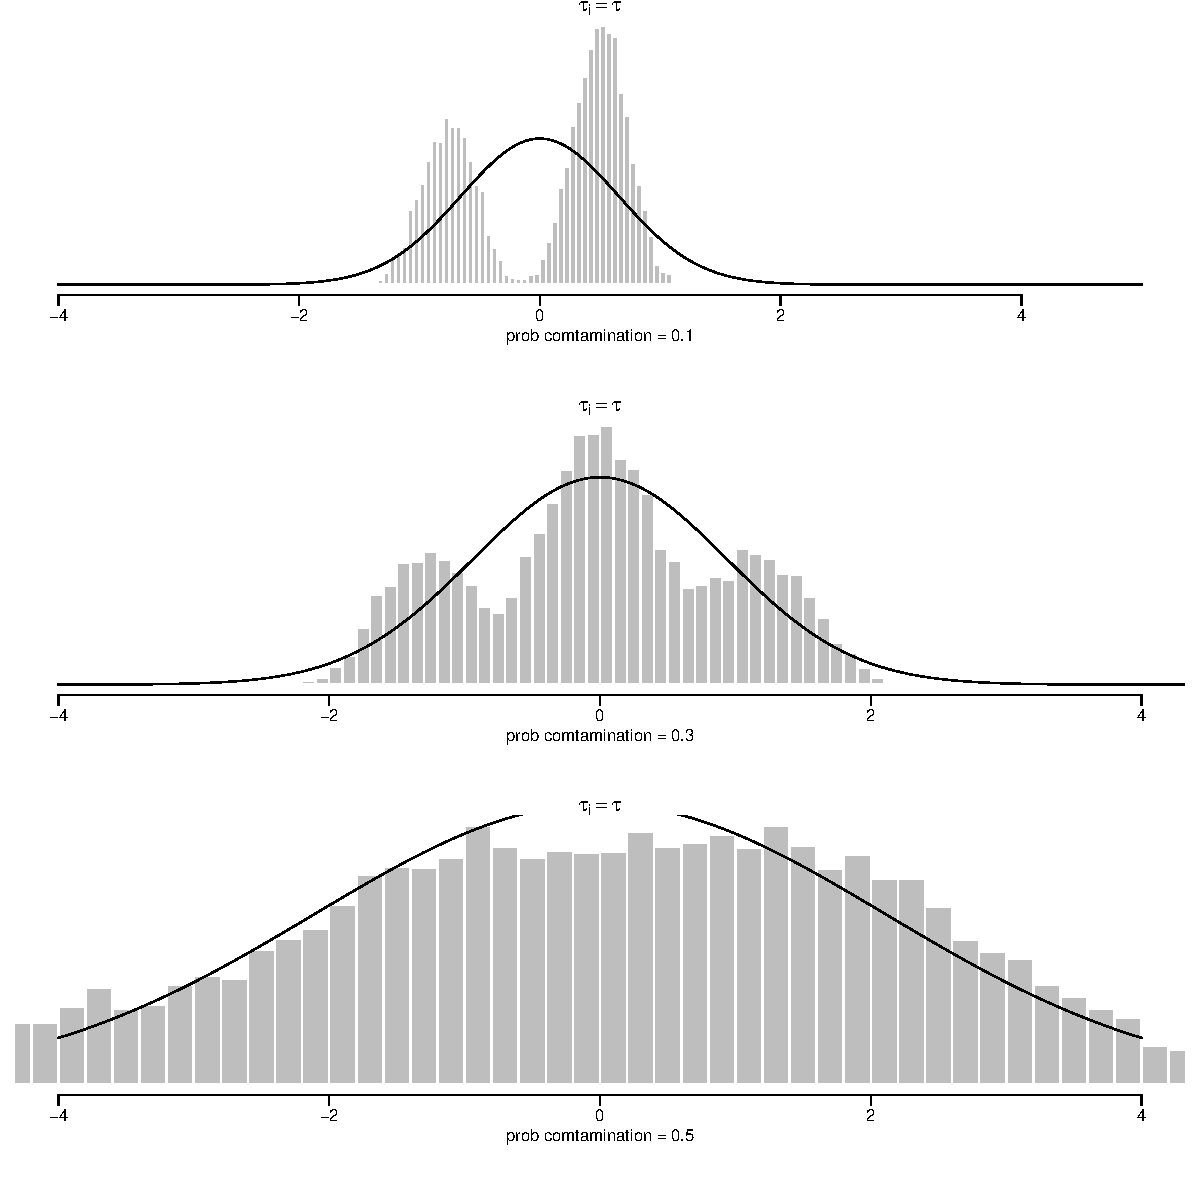
\includegraphics[width = \textwidth]{figures/neyman_comtamination_realized2.pdf}
 \caption{潜在结果受到不同概率污染时$\hat{\tau} - \tau$的抽样分布：第二次实现}\label{fig::simulation-neyman-heavytail-2}
 \end{figure} 
 
 


\subsection{实际数据应用}
\label{sec::example-neyman-formula}


第\ref{sec::frt-lalonde-experiment}节用\ri{lalonde}数据说明了 FRT，现在用同一数据说明本章理论。 
\begin{lstlisting}
> library(Matching)
> data(lalonde)
> z = lalonde$treat
> y = lalonde$re78
\end{lstlisting} 

利用定理\ref{thm::neyman1923}的公式，容易计算点估计与标准误：
\begin{lstlisting}
> n1= sum(z)
> n0= length(z) - n1
> tauhat = mean(y[z==1]) - mean(y[z==0])
> vhat   = var(y[z==1])/n1 + var(y[z==0])/n0
> sehat  = sqrt(vhat)
> tauhat
[1] 1794.343
> sehat
[1] 670.9967
\end{lstlisting} 

此结果与OLS所得估计量高度吻合。而使用EHW稳健标准误修正后所得置信区间则与内曼理论预期完全一致。 
\begin{lstlisting}
> olsfit = lm(y ~ z)
> summary(olsfit)$coef[2, 1: 2]
  Estimate Std. Error 
 1794.3431   632.8536 
 \end{lstlisting} 
但上述标准误比定理\ref{thm::neyman1923}给出的标准误小得多，可以通过 EHW 稳健标准误解决。 
\begin{lstlisting}
> library(car)
> sqrt(hccm(olsfit)[2, 2])
[1] 672.6823
> sqrt(hccm(olsfit, type = "hc0")[2, 2])
[1] 669.3155
> sqrt(hccm(olsfit, type = "hc2")[2, 2])
[1] 670.9967
 \end{lstlisting} 





\section{作业习题}

\paragraph{引理\ref{lemma::variancecovariancetau}的证明}\label{hw::proof-covariance-basic}


证明引理 \ref{lemma::variancecovariancetau}。 


\paragraph{定理\ref{thm::neyman1923}的另类证明}\label{hw::neyman-alternative-proof}


在完全随机实验下，计算
$$
\var\{  \hat{\bar{Y}}(1)  \} ,\quad
\var\{  \hat{\bar{Y}}(0)  \} ,\quad
\cov\{  \hat{\bar{Y}}(1) ,  \hat{\bar{Y}}(0)  \} 
$$
并据此计算$\var(\hat{\tau} )$。 

注：使用第\ref{chapter::SRS-appendix}章的结论。 





\paragraph{内曼推断与OLS}
\label{hw::neyman-ols-nox}


证明\eqref{eq::ols-difference-in-means}至\eqref{eq::ols-ehw}。此外，证明 EHW 稳健方差估计的 HC2 变体恰好恢复$\hat{V}$。 

注：第\ref{appendix::basic-linear-regression}章回顾了 OLS 的若干重要技术结论。
 
 



\paragraph{处理效应的异质性影响}\label{hw::treatment-effect-heterogeneity-neyman}


证明$S^2(\tau) = 0$蕴含$S^2(1) = S^2(0)$，并举出满足$S^2(1) = S^2(0)$但$S^2(\tau) \neq  0$的反例。 


证明$S^2(1) < S^2(0)$蕴含
$$
S(Y(0),\tau)  = (n-1)^{-1} \sumn \{ Y_i(0)  - \bar{Y}(0) \} (\tau_i - \tau) <0.
$$
并举出满足$S^2(1) > S^2(0)$但$S(Y(0),\tau)  < 0 .$的反例。



注：第一条说明，没有处理效应异质性就意味着处理与对照潜在结果的方差相等，但逆命题不成立。第二条说明，若处理潜在结果的方差小于对照潜在结果的方差，则个体处理效应与对照潜在结果负相关，逆命题同样不成立。相关讨论见\citet[][page 293]{gerber2012field}和\citet[][Appendix B.3]{ding2019decomposing}。 



\paragraph{方差估计式的优化}
\label{hw::better-bound-neyman}


\cite{Neyman:1923}的保守方差估计本质上采用了真实方差的上界
$$
\var(\widehat{\tau}) = \frac{S^2(1)}{n_1} + \frac{S^2(0)}{n_0} - \frac{S^2(\tau)}{n} \leq \frac{S^2(1)}{n_1} + \frac{S^2(0)}{n_0},
$$
这里使用了显然成立的$S^2(\tau) \geq 0$。证明另一个上界
\begin{eqnarray}\label{hw::cs-bound-neyman}
\var(\widehat{\tau})  \leq   \frac{1}{n} \left\{   \sqrt{  \frac{n_0}{n_1}  } S(1) +  \sqrt{  \frac{n_1}{n_0}  } S(0)   \right\}^2.
\end{eqnarray}
并说明\eqref{hw::cs-bound-neyman}何时取等号。 

根据上界\eqref{hw::cs-bound-neyman}，可构造另一个保守方差估计量
$$
\hat{V}' =  \frac{1}{n} \left\{   \sqrt{  \frac{n_0}{n_1}  } \hat S(1) +  \sqrt{  \frac{n_1}{n_0}  } \hat S(0)   \right\}^2.
$$
第\ref{sec::simulation-neyman-formula}节的模拟使用了$\hat{V}$。请重复模拟，加入方差估计量$\hat{V}' $及相应置信区间进行比较。 



注：证明时可参考第\ref{sec::cauchy-schwarz-inequality}节。上界\eqref{hw::cs-bound-neyman}还能改进；\citet{aronow2014sharp}利用 Fréchet--Hoeffding 不等式推导了$\var(\widehat{\tau}) $的尖锐上界。这些改进在实践中很少使用，主要有两个原因：一是比可方便地用 OLS 实现的$\hat{V}$复杂；二是基于$\hat{V}$的置信区间也适用于其他表述，例如结果对处理的真实线性模型，而这些改进一般不具备这种性质。因此，尽管理论上有趣，实际影响较小。 
 


\paragraph{\citet{Neyman:1923}定理的向量化拓展} \label{hw::vector-neyman1923}

\citet{Neyman:1923}的经典结论针对标量结果，实践中却常有多个结果。因此，将潜在结果推广为向量，考虑向量结果$\bm{V}  \in \mathbb{R}^K$上的平均因果效应：
$$
\tau_{\bm{V}} = \frac{1}{n}  \sumn \left\{  \bm{V}_i(1) - \bm{V}_i(0) \right\},
$$
其中$\bm{V}_i(1)$和$\bm{V}_i(0)$是单位$i$的$\bm{V}$潜在结果。$\tau_{\bm{V}}$的 Neyman 型估计量为处理组与对照组观测结果样本均值向量之差：
$$
\widehat{ \tau}_{\bm{V}} = \bar{\bm{V}}_1  - \bar{\bm{V}}_0 
= \frac{1}{n_1}   \sumn Z_i  \bm{V}_i   - \frac{1}{n_0}  \sumn (1-Z_i) \bm{V}_i . 
$$


考虑完全随机实验。证明$\widehat{ \tau}_{\bm{V}} $是$\tau_{\bm{V}} $的无偏估计，求$\widehat{ \tau}_{\bm{V}} $的协方差矩阵，并构造一个可能保守的方差估计量。 


\paragraph{完全随机实验下的统计推断}\label{hw::bre-inference}


探讨FRT在随机分配机制下的适用性，比较不同估计量及其渐近特性。 

\begin{definition}
[BRE]\label{def::BRE}
各处理指标$Z_i$独立同分布于 Bernoulli$(\pi)$，处理组人数为$n_1 = \sumn Z_i$，对照组人数为$n_0 = \sumn (1-Z_i)$。 
\end{definition}



首先，可以用 FRT 分析伯努利随机实验（BRE）。如何在 BRE 中检验$\HF$？若实际设计为 BRE，能否使用与完全随机实验相同的 FRT 程序？可以则说明依据，不可以则解释原因。

其次，可像\citet{Neyman:1923}分析完全随机实验那样，构造$\tau$的点估计及对应方差估计。 
\begin{enumerate}
\item
$\hat{\tau}$是$\tau$的无偏估计吗？是否一致？
\item
构造$\tau$的无偏估计量。
\item
比较上述无偏估计量的方差与$\hat{\tau}$的渐近方差。 
\end{enumerate}

注：在 BRE 下，估计量$\hat{\tau}$没有有限方差，但其渐近分布的方差有限。 



\paragraph{推荐阅读}

 \citet{Ding:2014}比较了分析完全随机实验的 Fisher 方法和 Neyman 方法。 


